\chapterimage{back2.jpg} % Chapter heading image
\chapter{Preface}
\label{preface}

This book provides an introduction to the CLEARSY Safety Platform (CSSP in short).
It is aimed at easing the development and the deployment of safety critical applications, up to SIL4. It is made of an integrated software development environment (IDE) and a hardware platform that natively integrates safety principles.
It relies on the smart integration of formal methods (including mathematical proof), redundant code generation and compilation, and a hardware platform that ensures a safe execution of the software.

The B formal method is at the core of the software development process. Mathematical proof ensures that the software complies with its specification (functional model) and guarantees the absence of programming errors while avoiding unit testing and integration testing. Moreover only one functional model is used to produce automatically the redundant software, avoiding the need to have two independent teams for its development \footnote{as required by railways standards for the highest SILs, for examples}.

The safety principles are built-in, both at software level and at hardware level (2oo2 hardware, 4oo4 software). They are out of reach of the developer who cannot alter them. The detection of any divergent behaviour among the two processors (PIC32 micro-controllers) and the four instances of the software is handled by the platform. The safety verification includes cross checks between software instances and between micro-controllers, memory integrity, ability to control outputs, etc. 

\begin{remark}
The CSSP Starter kits SK0 and SK1 are only for education and industrial prototyping respectively. If the software generated by the Atelier CSSP is the one that will be running on the final safety critical system, the electronics of SK0 and SK1 do not comply with SIL3 / SIL4 requirements. One of the reasons is that such electronics would largely increase the board prices and it would be clearly against the dissemination of the technology. \\
However the CSSP Core Module (available by the end of 2019), a daughter board to be plugged on a motherboard with digital IOs, will be SIL4-ready and usable in a real safety critical application.
\end{remark}

\section{Tool support}\index{Tool support}
Working with the CSSP \footnote{https://www.clearsy.com/en/our-tools/clearsy-safety-platform/} requires, as a minimum, access to the Atelier CSSP, an IDE derived from Atelier B \footnote{https://www.atelierb.eu/en/} and extended with specific features like diverse code generation and CSSP starter kit configuration. This IDE allows to create a CSSP project, specify and implement the behaviour of the CSSP, typecheck and compile the project. Finally the IDE allows to upload the program on the CSSP and to monitor its execution. For the execution of the program, either CSSP starter kit 0 (SK$_0$) or 1 (SK$_1$) board may be used. The only difference between the two boards are the number of digital IOs (5 for SK$_0$, 28 for SK$_1$). 


\section{Who this book is for}\index{Who this book is for}
This book is intended primarily as a textbook for post-graduates courses . It is also appropriate for courses on formal methods in general and on (safety related) embedded systems. The book assumes no prior knowledge of formal methods or of reasoning about programs. However it assumes a previous exposure to logic and a basic ability to manipulate simple logic and set theoretic expressions. No prior knowledge of the modelling language, namely the B language, is required as language elements will be introduced when needed. Moreover, as project skeletons are automatically generated, being able to develop a full B project is not required: programming the CSSP requires one component (the user\_logic operation) to be modified and possibly new components to be added. 

\section{To the instructor}\index{To the instructor}
This book has grown out of a course based around the B method and the CLEARSY Safety Platform, developed over a period of three years in Brazil, Canada, France, Italy, Portugal and UK.
The material is organised to introduce the central ideas as quickly as possible. This allows the students to become familiar with the tool support at the earliest possible stage, and to use it to develop their own programs. It also means that the students learn the B-method from a software engineering point of view, as they are taught from the viewpoint of using the B-method, rather than of the theory that underlies it. Such theory and language elements are introduced as and when they are needed. The Atelier CSSP generates a pre-filled B project, so the students do not need to develop a full B project but only to complete the specification and implementation of some CONSTANTS, VARIABLES, and OPERATIONS.
The first part of the book introduces the overall picture, the development process, and the language elements. They have to be read in this order.
The second part of the book contains a number of examples. The first two are related to synchronous and combinatorial programming, they have to be completed before moving to the next ones. \\

\noindent For any further information, requests or questions, please contact:
\begin{center}
contact-csp@clearsy.com    
\end{center}


\section{Book organisation}\index{Book organisation}

This book has an associated website, accessible from
\begin{center}
https://www.clearsy.com/en/our-tools/clearsy-safety-platform/    
\end{center}

\noindent This website contains the source code of all the examples and exercises presented in the book.

\section{Acknowledgements}\index{Acknowledgements}
The CLEARSY Safety Platform is being developed in order to compete on the international scene of safety critical systems, with the key idea to lower development and certification costs. Its development is a collective effort being produced in-house during development but also on site all over the world during deployment and exploitation, to obtain finally a safety, SIL4-ready product.\\
\\
We would like to thank people involved in the dissemination of the CLEARSY Safety Platform, allowing us to deliver talks, courses and hands-on sessions to their colleagues, either teachers, researchers or students, and in particular: Alexander Romanovsky (Univ. Newcastle, UK), Christiano Braga (UFF, Brazil), Emmanuel Chailloux (LIP6, France), Marc Frappier (Univ. Sherbrooke, Canada), Idir Ait Sadoune (CentraleSupelec, France), José Oliveira (Univ. Minho, Portugal), Leopoldo Teixeira (Univ. Pernambuco, Brazil), Marcel Oliveira (UFRN, Brazil), Tiago Massoni (Univ. Campina Grande, Brazil), Valerio Medeiros (IFRN, Brazil), and Yamine Ait-Ameur (Enseeiht, France). \\

\begin{figure}[h]
\centering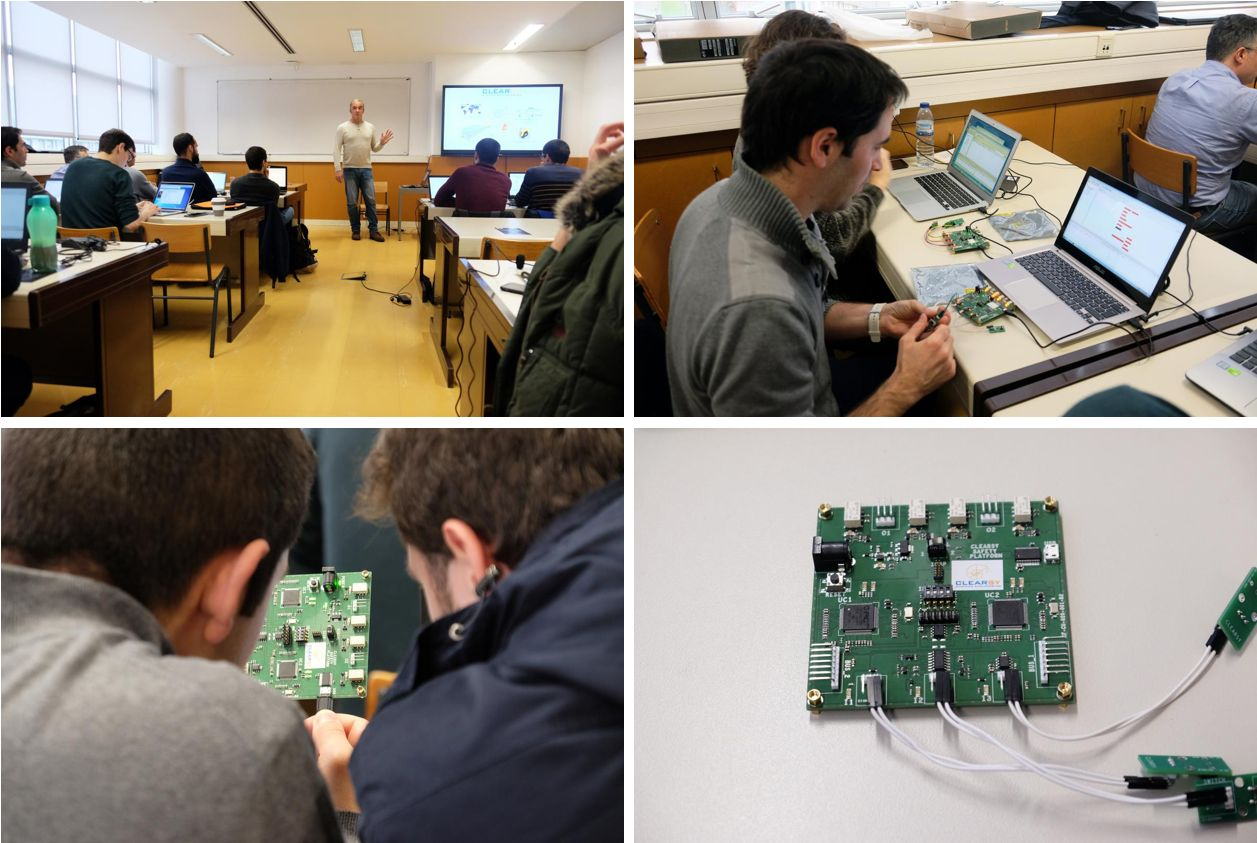
\includegraphics[scale=0.3]{Pictures/FOREWORD-TALK.jpg}
\caption{A busy hands-on session at the University of Minho in Braga, Portugal}
\end{figure}


Particular thanks are due to the team in charge of its development over the past years: Adrien Somoza, Bruno Lavaud, David Deharbe, Denis Sabatier, Eliott Trotebas, Emine Aktepe, Etienne Prun, Florent Patin, Guillaume Pressouyre, Hector Ruiz Barradas, José Tarsitano, Lilian Burdy, Loïc Claudet, Ludovic Delfau, Manfred Winkler, Mathieu Comptier, Maxime Renaud, Patrick Sauvage, Sébastien Agostini, Sylvain Breux, Thierry Lecomte, Thomas Gonthier, Vivien Galuchot.\\

%
\hspace*{\fill} Aix en Provence, France, July 2019
